\documentclass{article}
\usepackage{graphicx} % Required for inserting images
\usepackage{listings}
\usepackage{float}
\usepackage{color}
\usepackage{booktabs} 
\definecolor{codegreen}{rgb}{0,0.6,0}
\definecolor{codegray}{rgb}{0.5,0.5,0.5}
\definecolor{codepurple}{rgb}{0.58,0,0.82}
\definecolor{backcolour}{rgb}{0.95,0.95,0.92}
\usepackage[numbers]{natbib}
\usepackage{hyperref}

\lstdefinestyle{mystyle}{
    backgroundcolor=\color{backcolour},   
    commentstyle=\color{codegreen},
    keywordstyle=\color{magenta},
    numberstyle=\tiny\color{codegray},
    stringstyle=\color{codepurple},
    basicstyle=\footnotesize,
    breakatwhitespace=false,         
    breaklines=true,                 
    captionpos=b,                    
    keepspaces=true,                 
    numbers=left,                    
    numbersep=5pt,                  
    showspaces=false,                
    showstringspaces=false,
    showtabs=false,                  
    tabsize=2
}

\lstset{style=mystyle}


\begin{abstract}

In recent years, leveraging satellite imagery with deep learning (DL) architectures has become an effective approach for environmental monitoring tasks, including forest wildfire detection. Nevertheless, this integration requires substantial high-quality labeled data to train the DL models accurately. Leveraging the capabilities of multiple Python libraries, such as rasterio and GeoPandas, and Google Earth Engine’s Python API, this study introduces a streamlined methodology to efficiently gather, label, augment, process, and evaluate a large-scale bi-temporal high-resolution satellite imagery dataset for DL-driven forest wildfire detection. Known as the California Wildfire GeoImaging Dataset (CWGID), this dataset comprises over 100,000 labeled 'before' and 'after' wildfire image pairs, created from pre-existing satellite imagery. An analysis of the dataset using pre-trained and adapted Convolutional Neural Network (CNN) architectures, such as VGG16 and EfficientNet, achieved accuracies of respectively 76\% and 93\%. The pipeline outlined in this paper demonstrates how Python can be used to gather and process high-resolution satellite imagery datasets, leading to accurate wildfire detection and providing a tool for broader environmental monitoring.

\end{abstract}

\section{Introduction}\label{introduction}
 

This paper presents a Python-based methodology for gathering and using a labeled high-resolution satellite imagery dataset for forest wildfire detection. 

Forests are important ecosystems found globally. They are made up of trees, plants, and other various types of vegetation. Forests host many species and are crucial for maintaining environmental health, as they support biodiversity, climate regulation, and oxygen production. Moreover, they bring economic and social benefits, including energy production, job opportunities, and spaces for leisure and tourism. Protecting forests and tackling forest loss is a current global priority \citep{IUCN2021}.

With the development of Earth Observation (EO) systems, remote sensing became a time-efficient and cost-effective method for monitoring and detecting forest change \citep{Massey2023}. Moreover, recent advancements in satellite technology have significantly enhanced forest monitoring capabilities by providing high-resolution imagery and increasing the frequency of observations. 

Satellite imagery-based change detection and forest monitoring have traditionally relied on manually identifying specific features and using predefined algorithms and models, such as differential analysis, thresholding techniques, and clustering and classification algorithms. This approach requires considerable domain expertise and such algorithms and models may not capture the full complexity of the studied data \citep{rs14071552}. 

With the emergence of deep learning (DL) algorithms, specifically computer vision methods, such as Convolutional Neural Networks (CNNs) \citep{lecun} and Fully Convolutional Neural  Networks (e.g., U-Nets \citep{DBLP:RonnebergerFB15}), there is a significant opportunity to enhance and facilitate forest change detection efforts. These advanced computational methods can rapidly identify complex patterns within vast datasets. Furthermore, when integrated with EO systems they can facilitate near real-time monitoring and detection of multiple forest loss causes, assess their extent, or even predict and evaluate their spread \citep{eleo,al-dabbagh2023uni}. Thus, integrating DL methods with satellite imagery offers a more dynamic and precise approach, capable of handling the patterns and variability associated with imagery data. For instance, DL models can automatically learn complex patterns related to wildfire spread from labeled examples, whereas traditional methods might miss subtle but important indicators. 

However, DL algorithms require a substantial amount of labeled data to effectively learn and identify change \citep{Alzubaidi2021ReviewOD}. Therefore, the development of labeled high-resolution satellite imagery datasets is important and relevant for addressing environmental problems. Currently, the availability of labeled high-quality satellite imagery datasets is an obstacle to developing DL models for environmental change detection \citep{Adegun2023}. 

Generally, building a satellite imagery dataset is a time-intensive process. However, Google Earth Engine (GEE) \citep{gorelick2017google} has recently revolutionized this process by providing an extensive, cloud-based platform for the efficient collection, processing, and analysis of satellite imagery. GEE’s Python API allows its users to programmatically query their platform and download cloud-free large-scale satellite imagery datasets from multiple satellite collections, such as Sentinel-2. 

For example, while traditional methods might require manual search and download of images, GEE can automate this process, significantly reducing the time needed to find suitable satellite images. This technology makes data collection and processing faster and easier, facilitating environmental monitoring by providing reliable and easily accessible high-quality satellite imagery.

Furthermore, Python facilitates the use of DL in environmental monitoring by providing a rich ecosystem of libraries and tools, such as TensorFlow \citep{tensorflow2015-whitepaper}, which contains multiple existing DL architectures that can be adapted and used with satellite imagery. Nevertheless, integrating DL and remotely sensed images requires multiple processing steps, such as having smaller imagery tiles and adapting the models to use GeoTIFF data, among others. These steps include:
\begin{enumerate}
    \item Data Acquisition: Collect satellite imagery from sources such as Google Earth Engine or 		 other satellite image providers.
    \item Image Tiling: Divide large satellite images into smaller tiles to fit the input image size used in DL models.
    \item Data Annotation: Label the images to create a ground truth dataset for training DL models.
    \item Data Augmentation: Applying transformations such as rotations and flips to increase the diversity of the training dataset.
\end{enumerate}
Python’s tools help manage these steps. For example, libraries like rasterio, Tifffile and GeoPandas, can be used to process and transform satellite imagery data into formats suitable for DL models.


This paper presents a methodology, implemented in Python, to streamline the creation and evaluation, via DL, of satellite imagery datasets. The methodology covers the entire workflow: from data acquisition, labelling, and preprocessing to model adaptation, training, and evaluation. Specifically, this approach is applied to gather and validate a high-resolution dataset for forest wildfire detection, the California Wildfire GeoImaging Dataset (CWGID). Additionally, this methodology can be adapted for various environmental monitoring tasks, showing its versatility in studying and responding to different environmental changes.


\section{Building a Sentinel-2 Satellite Imagery Dataset}
To construct the CWGID, a multi-step process is needed. 
\subsection{Gathering and Refining Historic Wildfire Polygon Data from California}
The initial step is to gather georeferenced forest wildfire polygon data from California, sourced from the Fire and Resource Assessment Program (FRAP) maintained by the California Department of Forestry and Fire Protection \citep{california_department_of_forestry_and_fire_protection_2024}. This FRAP data includes perimeters of past wildfires and serves as the geographic reference needed to select satellite imagery with GEE. Figure \ref{fig2} illustrates the polygons from the FRAP. The polygons delineated in purple represent areas affected by wildfires in forested regions. These delineated polygons are used to create the CWGID. 


\begin{figure}[h]
    \centering
    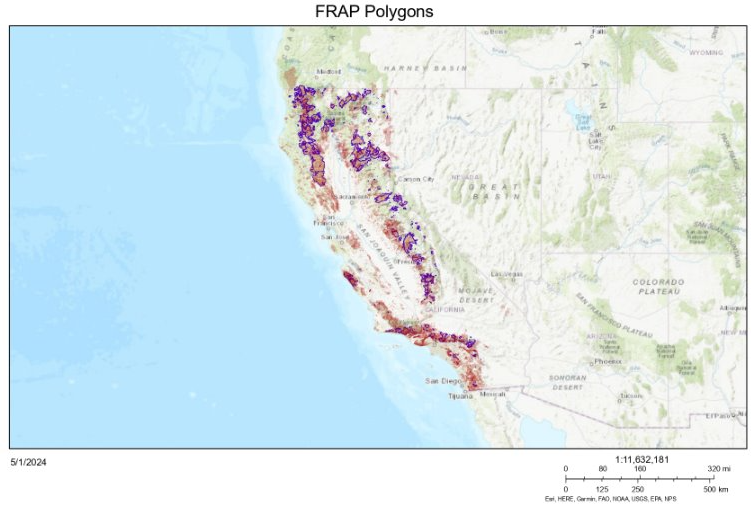
\includegraphics{polygons.png}
    \caption{Representation of the Polygon Data from the FRAP. Polygons delineated in purple represent wildfires that occurred in forested areas, used for the California Wildfire GeoImaging Dataset (CWGID). \label{fig2}}
\end{figure}

Then, in Python, the Pandas library \citep{pandas1} is used to organize the forest wildfire attribute data into a Pandas DataFrame, which is then filtered to align with the launch date and operational phase of the Sentinel-2 satellites, selected for their open-source, high-resolution imagery capabilities \citep{DRUSCH201225}. Additionally, the dates are adjusted to fall within the green-up period, avoiding the winter and fall seasons where snow cover could interfere with identifying burnt areas.

Next, the data is formatted to meet GEE’s querying specifications:
\begin{itemize}
    \item A 15-day range for pre- and post-wildfire dates is generated and added to the DataFrame.
    \item Using Pandas, the date ranges are formatted to meet GEE's requirements.
    \item Using the pyproj library \citep{pyproj2023}, the recorded point coordinates are converted from NAD83 to WGS84 to facilitate the querying process.
    \item With the geopy \citep{geopy} library, the coordinates of the squared region of interest are calculated, featuring a side length of 15 miles.
\end{itemize}


\subsection{Downloading the Imagery Data Using GEE's Python API}
GEE is a cloud-based platform for global environmental data analysis. It combines an extensive archive of satellite imagery and geospatial datasets with powerful computational resources to enable researchers to detect and quantify changes on the Earth’s surface. GEE’s Python API offers an accessible interface for automating the process of satellite imagery downloads, making it a popular tool for environmental monitoring and research projects.

Multiple steps are needed to set up the GEE's Python API. First, a project is created in Google Cloud Console and the Earth Engine API is enabled. Authentication and Google Drive editing rights are configured to effectively manage and store the downloaded imagery. Following the setup, the Earth Engine Python API is installed on a local machine, and the necessary authentications are performed to initialize the API. 

Then, a Python script is developed to automate the download of images depicting the pre- or post-wildfire data using GEE's Python API (see Code \ref{download}). To download three-channel RGB GeoTIFF imagery, the bands B4 (red), B3(green), and B2(blue) need to be specified (different band compositions can be selected in this step). In satellite imagery, bands refer to specific wavelength ranges captured by the satellite sensors, and they are used to create composite images that highlight different features of the Earth's surface. These bands correspond to the visible spectrum, which is useful for visual interpretation and analysis.
The script to download the satellite imagery needed using GEE (see Code \ref{download}) is configured with a for loop to iterate through each entry in the DataFrame, extracting necessary parameters such as date ranges, region of interest (ROI) coordinates, and center coordinates of each wildfire polygon. Also, the script is designed to specify parameters such as the desired image collection and a threshold for cloud coverage. Tiles exhibiting more than 10\%  cloud coverage are automatically excluded to maintain data quality. Finally, the images are downloaded and exported to Google Drive in a GeoTIFF format. 

\begin{lstlisting}[language=Python, label=download, caption=Script to automate the download of pre- or post-wildfire images using GEE’s Python API. It iterates through a DataFrame, extracting relevant parameters and downloading images with less than 10\% cloud coverage. The images are exported as GeoTIFF files to Google Drive.]
# Authenticate into EE
ee.Authenticate()

# Initialize EE
ee.Initialize()

# Initialize a list for iteration
indices = []
for i in range(0, x):  # modify depending on your number of data points
    indices.append(i)

# Define the bands you want to download
bands_rgb = ['B4', 'B3', 'B2']  # Red, Green, Blue

event_type = 'before'  # Toggle this to 'after' as needed

for i in indices:
    # Set the center point of the wildfire polygon
    center_point = ee.Geometry.Point(round(data[i][1], 2), round(data[i][2], 2))

    # Select an image from the specified satellite collection for the center point
    tile = ee.ImageCollection('COPERNICUS/S2') \  # Define the satellite imagery you will be working with, in this case Sentinel 2
        .filterBounds(center_point) \
        .filterDate(data[i][3], data[i][4]) \  # Define a date range for the satellite image
        .sort('CLOUDY_PIXEL_PERCENTAGE') \  # Organize the images based on the % cloud cover
        .first()  # Get the image with the lowest cloud cover

    # Check the properties of the image
    image_properties = tile.getInfo()
    cloudy_percentage = image_properties.get(
        'properties', {}).get('CLOUDY_PIXEL_PERCENTAGE', 0)  # Obtain the exact percentage of cloud cover for each image

    # Proceed if the image has less than 10% cloud coverage
    if cloudy_percentage <= 10: 
        # Define the Region of Interest (ROI) using the provided coordinates
        roi = ee.Geometry.Polygon([[
            [data[i][9], data[i][10]],
            [data[i][11], data[i][12]],
            [data[i][13], data[i][14]],
            [data[i][15], data[i][16]],
            [data[i][17], data[i][18]]]])

        # Select the RGB bands from the image
        rgb_tile = tile.select(bands_rgb)

        # Export RGB image to Google Drive
        rgb_task = ee.batch.Export.image.toDrive(**{
            'image': rgb_tile,
            'description': f'RGB_{event_type}Fire'
            + str(data[i][0]),  # Descriptive name for the task
            'folder': f'GEE_FireImagesRGB_{event_type}',  # Folder in Google Drive to save the image
            'scale': 10,  # Adjust the scale as needed
            'region': roi.getInfo()['coordinates'],  # Region of Interest for the export 
            'crs': 'EPSG:4326',  # Coordinate reference system
            'fileFormat': 'GeoTIFF',  # File format for the export
        })
        rgb_task.start()

        # Monitor the task status until it completes or fails
        while not rgb_task.status()['state'] in ['COMPLETED', 'FAILED', 'CANCELLED']:
            print(f'RGB Task for {event_type} fire is', rgb_task.status()['state'])
            # Add a short wait before checking again

        # Check the final task status
        rgb_task_status = rgb_task.status()
        print(f"RGB Task Status for {event_type} fire:", rgb_task_status)
        print(f"RGB Task Error Message for {event_type} fire:", rgb_task_status.get("error_message", "No error message"))
    else:
        # Skip images with more than 10% cloud coverage
        print(f"Skipping image {i} due to cloudy percentage ({cloudy_percentage} %) > 10 %")
\end{lstlisting}


Figure \ref{fig3} presents an example of a pre-and post-wildfire imagery pair downloaded from GEE to Google Drive using code \ref{download} . 

\begin{figure}[H]
    \centering
    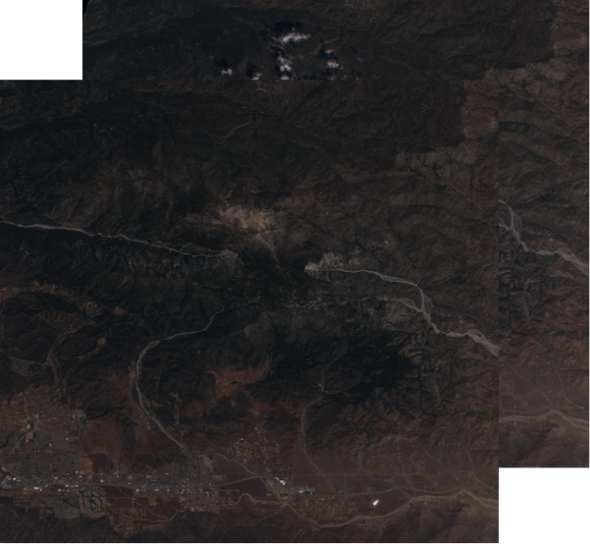
\includegraphics{prepost1.png}
    \caption{Example of a  pre and post-wildfire RGB image pair of a forested area downloaded using GEE's Python API. \label{fig3}}
\end{figure}
\subsection{Creating the Ground Truth Wildfire Labels}
Ground truth masks are essential in forest wildfire detection and general land cover classifications \citep{8113128}. In this project, these type of masks are generated to label the data.

First, Python is used to rasterize the combined geometry of the forest wildfire polygon data and the downloaded post-wildfire RGB satellite imagery. Specifically, the forest wildfire polygons are accessed in Python using GeoPandas \citep{geopandas} and reprojected to match the coordinate system of the satellite imagery (EPSG:4326). Then, each post-wildfire RGB image is locally and temporarily downloaded from Google Drive, with essential properties such as width, height, transform, and bounds extracted using the rasterio library \citep{rasterio}. Next, the geometry column from the forest wildfire polygon data is extracted and intersected with each image bound using Python's shapely \citep{shapely} library. Finally, binary masks are created by rasterizing the combined geometries. These masks match the dimensions of the satellite images, ensuring that each pixel labeled as wildfire damage corresponds directly to the polygon data (see Code \ref{lst:fire_polygons_processing}). The binary masks are saved temporarily in GeoTIFF format and are uploaded to a dedicated Google Drive folder.  All the temporary local files were deleted to clear space and maintain system efficiency.  
\begin{lstlisting}[language=Python, label= lst:fire_polygons_processing, caption = Building Ground Truth Masks]
import geopandas as gpd
import numpy as np
import rasterio
from shapely.geometry import box, shape
import os

# Define the path to your Shapefile - replace with your specific path
shapefile_path = "YourShapefileDirectory/FirePolygons.shp"

# Read the Shapefile using geopandas
gdf = gpd.read_file(shapefile_path)

# Reproject the shapefile to EPSG:4326 to match the satellite imagery coordinate system
gdf = gdf.to_crs(epsg=4326)

# Create a directory to store the output raster masks if it doesn't already exist
output_dir = "raster_masks"
if not os.path.exists(output_dir):
    os.makedirs(output_dir)

# Iterate through the rows in the attribute table
for index, row in gdf.iterrows():
    object_id = row["OBJECTID"]
    image_path = f"YourImageDirectory/RGB_AfterFire{object_id}.tif"
    # Check if the image exists
    if os.path.exists(image_path):
        # Open the image using rasterio
        with rasterio.open(image_path) as src:
            image_width = src.width
            image_height = src.height
            image_transform = src.transform
            image_bounds = box(
                src.bounds[0], src.bounds[1],
                src.bounds[2], src.bounds[3]
            )

        # Extract the geometry column
        geom = shape(row["geometry"])
        clipped_geom = geom.intersection(image_bounds.envelope)

        if not clipped_geom.is_empty:
            # Create a two-dimensional label by rasterizing the
            # clipped geometry
            clipped_mask = rasterio.features.geometry_mask(
                [clipped_geom],
                out_shape=(image_height, image_width),
                transform=image_transform,
                invert=True,
            )

            # Save the image with the two-dimensional label overlay
            output_image_path
            = f"{output_dir}/Masked_{object_id}.tif"
            with rasterio.open(
                output_image_path,
                "w",
                driver="GTiff",
                width=image_width,
                height=image_height,
                count=1,
                dtype=np.uint8,
                crs=src.crs,
                transform=image_transform,
            ) as dst:
                dst.write(clipped_mask.astype(np.uint8), 1)
\end{lstlisting}

In the resulting ground truth masks, the pixel values are set to zero if they are outside of a wildfire polygon, indicating unaffected areas, and set to one if they are within the polygon boundaries, indicating areas affected by a forest wildfire. Figure \ref{fig4} displays an example of a resulting ground truth mask.


\begin{figure}[H]
    \centering
    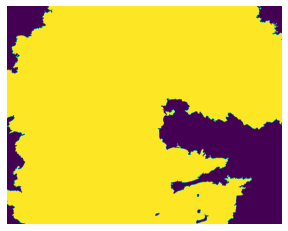
\includegraphics{label1.png}
    \caption{Example of a resulting ground truth mask in a forested area affected by wildfires. The mask highlights wildfire-affected areas in yellow and unaffected areas in purple. This binary mask is used to train and validate deep learning models for accurate wildfire detection \label{fig4}}
\end{figure}


\subsection{Image Segmentation and Data Preparation for Deep Learning Architectures}
Next, the satellite images and their corresponding ground-truth masks are cropped into smaller tiles that maintain the imagery's spatial resolution (10m). Often, satellite imagery needs to be resized and downscaled to accommodate deep learning (DL) architectures, which can result in the loss of essential details such as subtle indicators of early-stage wildfires. Moreover, using smaller images enhances the efficiency of DL models by lowering computational demands and speeding up training times \citep{hu2015transferring,marmanis2016deep}. 

To do this, a tile size of 256x256 pixels is specified and each RGB image is downloaded individually from Google Drive to a temporary local folder. Using Python’s rasterio library, the original RGB images are opened to obtain their dimensions. Then, the number of rows and columns for the tiles is calculated based on the chosen tile size. Next, a rasterio Window object is used to extract the corresponding portion from the original image and read the RGB data, ensuring the order of the bands (B4, B3, and B2).

The segmented RGB tiles are then saved as GeoTIFF files using the tifffile Python library \citep{tifffile}. This is a critical step to maintain the integrity of the three-channel RGB data, as the rasterio library alone can alter the color of the images during saving. Additionally, the metadata of the saved tiles is updated to include georeferencing information and to modify parameters such as width, height, and transform (see Code \ref{lst:save_rgb_tiles}).

A similar approach is used to segment the binary masks, specifying that the images contain only one band. 
\begin{lstlisting}[language=Python, caption={Function to Crop RGB Image Tiles}, label= lst:save_rgb_tiles]
from rasterio import Window
from tifffile import imwrite

# Function to save image tiles without changing the data type
def save_rgb_tiles(image_path, output_folder, tile_size, parent_name):
    # Open the source image file 
    with rasterio.open(image_path) as src:
        height = src.height # Get the height of the source image
        width = src.width # Get the width of the source image
        
        # Calculate the number of tiles in both dimensions
        num_rows = height // tile_size
        num_cols = width // tile_size

        tile_counter = 1  # Initialize the tile counter
        
        # Iterate over the number of rows of tiles
        for i in range(num_rows):
            # Iterate over the number of columns of tiles
            for j in range(num_cols):
                # Define the window for the current tile
                window = Window(j * tile_size, i * tile_size, tile_size, tile_size)

                # Read the original data without modifications
                # Assuming band order B4, B3, B2
                tile = src.read((1, 2, 3), window=window)
                # Create a unique name for the tile
                tile_name = f"{parent_name}_tile_{tile_counter}.tif"
                # Define the path to save the tile
                tile_path = os.path.join(output_folder, tile_name)

                # Save the tile using tifffile without changing
                # data type
                imwrite(tile_path, tile)

                # Copy the metadata from the source image
                meta = src.meta.copy()
                # Get the transformation matrix for the current window
                transform = src.window_transform(window)
	    	    # Update the metadata with the new dimensions and transformation
                meta.update({
                    'width': tile_size,
                    'height': tile_size,
                    'transform': transform
                })
	            # Save the tile with updated metadata using rasterio
                with rasterio.open(tile_path, 'w', **meta) as dst:
                    dst.write(tile)
                tile_counter += 1  # Increment the tile counter
\end{lstlisting}

\begin{figure}[H]
    \centering
    \includegraphics[width=0.9\textwidth]{crop.png}
    \caption{Example of cropped pre- and post-wildfire images and their corresponding label}. \label{figcrop}
\end{figure}

By combining the capabilities of rasterio for efficient geospatial data handling and the tifffile library for preserving the RGB data during saving, the original images are cropped into smaller RGB tiles. This approach preserves the resolution and the georeferencing information of the images, preparing them to train DL applications.
\subsection{Data Augmentation for Wildfire Damage Detection}
It is essential to have a balanced dataset that includes both forest wildfire-affected and unaffected areas. Initially, the dataset comprised 82,082 tiles, but only 4,847 of these showed signs of wildfire damage, indicating a significant class imbalance. This could lead to overfitting, with the model biased towards undamaged landscapes.

To address this imbalance and enhance the model's accuracy in detecting wildfire-affected areas, data augmentation techniques are implemented. Specifically, functions using the rasterio and NumPy \citep{numpy} libraries are developed to perform image transformations, which include rotating the GeoTIFF tiles by 90°, 180°, and 270°, and flipping them horizontally and vertically. These transformations are applied to the imagery and the mask tiles that contain fire polygons and to their corresponding pre-wildfire RGB GeoTIFF tiles.

Finally, the augmentation process increased the diversity of the training data and resulted in a total of 106,317 pairs of labeled RGB GeoTIFF image tiles, with 29,082 positive instances (wildfire damage), improving the class balance.

Figure \ref{fig0} illustrates the data augmentation process applied to the satellite imagery. The original image tile is shown alongside its augmented versions, which include rotations and flips. This augmentation increases the diversity of the dataset, helping to balance the classes and improve the model's ability to detect wildfire-affected areas accurately.
\begin{figure}[H]
    \centering
    \includegraphics{augment.png}
    \caption{Representation of the data augmentation performed to the 256px*256px tiles to increase positive examples of wildfire damage. \label{fig0}}
\end{figure}

\section{Evaluating the CWGID Using Convolutional Neural Networks}
The CWGID is tested for demonstration purposes using the well-known CNN architectures VGG16 and EfficientNet, both implemented using Python's TensorFlow’s Keras API. It is important to mention that both models were executed locally on a MacBook Pro equipped with a 2.4 GHz Intel Core i9 processor and 16 GB of 2400 MHz DDR4 memory.

Satellite image data usually requires significant storage and processing power because each image contains a large amount of data across the chosen spectral bands and stores important geographic information. Hence, the scale and speed of model training observed in the results below is constrained. 

For users with access to high-performance computing clusters or cloud-based GPU instances, processing times can significantly reduce.

\subsection{VGG16 Implementation}
VGG16 \citep{Simonyan15} is a deep CNN designed for image processing and classification tasks. It consists of 13 convolutional layers, 5 pooling layers, and 3 fully connected layers. This model is adapted to train on the dataset and detect positive and negative instances of forest wildfires. The VGG16 architecture only trains on the post-wildfire 3-channel RGB imagery (i.e., images collected prior to the wildfire were not used with VGG16), which contains both. 

To use this CNN architecture with GeoTIFF satellite images, which typically store geographic data not supported by most deep-learning libraries, a custom function is implemented to process and feed the data to the model using the rasterio library and the shuffle function from the Scikit-learn library \citep{sklearn1,sklearn2}. This function (see Code \ref{lst:custom_generator}) is crucial for handling the unique structure of GeoTIFF files and converting them into a format suitable for deep learning. It is designed to read batches of GeoTIFF files, shuffle them to ensure randomness, and process them into a three-dimensional array compatible with VGG16. Here is how it works:

\begin{itemize}
\item File Paths Initialization: The function starts by taking the file paths of the GeoTIFF images and shuffling them using the shuffle function from Scikit-learn to ensure the batches are randomly ordered.

\item Batch Processing: It processes the images in batches of 32 files. For each batch, the function initializes empty lists for images and labels.

\item Reading and Transforming Images: It reads each GeoTIFF file using rasterio. The images are then transformed to have the channels last (i.e., changing the format from \textbf{channels, height, width} to \textbf{height, width, channels}) to use with Keras.

\item Labels are assigned based on the presence of "Damaged" in the file paths. Specifically, if the file path contains the string "/Damaged/", the image is labeled as 1 (indicating it shows a damaged area). If the file path does not contain this string, the image is labeled as 0 (indicating it shows an undamaged area). In this method, the ground-truth masks are not directly used but are leveraged to define the imagery file paths. 

\item Yielding Batches: Finally, the function yields batches of images and labels as Numpy arrays, which are then fed into the VGG16 model for training.
\end{itemize}


\begin{lstlisting}[language=Python, caption={Custom Function to Feed GeoTIFF Files to the VGG16 Model: The function reads batches of 32 GeoTIFF files, shuffles them, and processes them into a three-dimensional array compatible with VGG16.}, label= lst:custom_generator]
from sklearn.utils import shuffle

# Define the base paths for training and testing
base_training_path = "Insert your training file path"
base_testing_path = "Insert your testing file path"

def custom_image_generator(file_paths, batch_size):
    while True:
        file_paths = shuffle(file_paths)

        for i in range(0, len(file_paths), batch_size):
            batch_files = file_paths[i : i + batch_size]
            images, labels = [], []

            for file in batch_files:
                with rasterio.open(file) as src:
                    image = src.read()
                    # Channels last
                    image = np.moveaxis(image, 0, -1)

                label = 1 if "/Damaged/" in file else 0
                images.append(image)
                labels.append(label)

            yield np.array(images), np.array(labels)
\end{lstlisting}

To detect wildfire-affected areas with VGG16, the model is initiated using the pre-trained weights from the ImageNet dataset. The convolutional base is frozen to preserve the integrity of the learned features and to focus on the training of the added layers. A Flatten operation is applied to the output to transform the two-dimensional feature maps into a one-dimensional vector. Then, a fully connected dense layer with 512 neurons, L2 regularization, and ReLU activation is added. A Dropout layer with a rate of 0.5 is included to further prevent overfitting. Finally, the network becomes a single-neuron dense layer with a sigmoid activation function that produces a probability score of wildfire damage. Before training, class weights are calculated using the Scikit-learn library. 
Furthermore, Keras callbacks are set up for early stopping and model checkpointing to avoid overfitting.

The complete model is compiled with the Adam optimizer \citep{kingma2014adam}, binary cross-entropy loss \citep{goodfellow2016deep}, and accuracy, precision, and recall as the performance metrics (see Code \ref{lst:vgg16_wildfire_detection}). The Adam optimizer is chosen because it adapts the learning rate during training. In the context of satellite image classification, where the landscape can vary significantly across images, Adam’s ability to adjust the learning rate is important. Also, the binary cross-entropy loss is chosen because it is tailored for binary classification tasks, such as classifying between damaged and undamaged forested areas in satellite images.

\begin{lstlisting}[language=Python, caption={Adaptation of VGG16 for Wildfire Damage Detection}, label= lst:vgg16_wildfire_detection]
from keras.models import Model
from keras.layers import Flatten, Dense
from keras.optimizers import Adam
from keras.applications import VGG16
from keras.metrics import Precision, Recall

# Define the base model using pre-trained ImageNet weights
base_model = VGG16(weights='imagenet', include_top=False, input_shape=(256, 256, 3))

# Freeze the convolutional base to prevent weights from being updated
for layer in base_model.layers:
    layer.trainable = False

# Add custom layers on top of the base model
x = Flatten()(base_model.output) # Flatten the output to make it suitable for dense layers
x = Dense(512, activation='relu', kernel_regularizer='l2')(x) # Add a dense layer with 512 units, L2 regularization and ReLU activation
output = Dense(1, activation='sigmoid')(x) # Output layer with a sigmoid activation for binary classification

# Construct the complete model
model = Model(inputs=base_model.input, outputs=output)

#Callbacks to prevent overfitting
early_stopping = EarlyStopping(monitor='val_loss', patience=3, restore_best_weights=True)
model_checkpoint = ModelCheckpoint('best_modelVGG16.keras', monitor='val_loss', save_best_only=True)

# Compile the model with Adam optimizer and binary cross-entropy loss
model.compile(optimizer=Adam(learning_rate=0.0001),
              loss='binary_crossentropy',
              metrics=['accuracy', Precision(), Recall()])

\end{lstlisting}

The VGG16 model is trained and validated on 49313 three-channel RGB images (divided as follows: 90\% for training and 10\% for validation) and is tested on 5479 images. Training took around 1010 minutes for 10 epochs. The detailed training and validation performance metrics for each epoch are provided in Table \ref{tab:vgg}. The graphs showing the changes of the training and validation metrics over the 10 epochs can be seen in Figure \ref{figvgg}.

\begin{table}[H]
    \centering
    \caption{Performance Metrics for Training and Validation Sets Using VGG16 Across Epochs. \label{tab:vgg}}
    \begin{tabular}{ccccccc}
    \toprule
    \textbf{Epoch} & \textbf{Training Accuracy} & \textbf{Training Precision} & \textbf{ Training Recall} & \textbf{Validation Accuracy} & \textbf{Validation Precision} & \textbf{Validation Recall} \\
    \midrule
    1/10 & 0.6729 & 0.7241 & 0.6229 & 0.7291 & 0.7689 & 0.6812 \\
    2/10 & 0.7406 & 0.7892 & 0.6992 & 0.7471 & 0.7716 & 0.7256 \\
    3/10 & 0.7537 & 0.8079 & 0.7052 & 0.7473 & 0.7729 & 0.7261 \\
    4/10 & 0.7555 & 0.8306 & 0.6788 & 0.7541 & 0.7899 & 0.7155 \\
    5/10 & 0.7568 & 0.8354 & 0.6765 & 0.7543 & 0.8070 & 0.6906 \\
    6/10 & 0.7632 & 0.8439 & 0.6813 & 0.7539 & 0.8226 & 0.6655 \\
    7/10 & 0.7653 & 0.8514 & 0.6768 & 0.7569 & 0.8049 & 0.6998 \\
    8/10 & 0.7661 & 0.8504 & 0.6803 & 0.7635 & 0.8228 & 0.6887 \\
    9/10 & 0.7680 & 0.8536 & 0.6808 & 0.7504 & 0.8771 & 0.6008 \\
    10/10 & 0.7692 & 0.8622 & 0.6742 & 0.7527 & 0.8164 & 0.6760 \\
    \bottomrule
    \end{tabular}
\end{table}
During the training process, the model’s performance on the training set showed a consistent increase in accuracy, precision, and recall. Specifically, the training accuracy improved from 0.6729 in the first epoch to 0.7692 in the tenth epoch. The precision increased from 0.7241 to 0.8622, and the recall fluctuated but overall showed an upward trend, starting at 0.6229 and ending at 0.6742.

\begin{figure}[H]
    \centering
    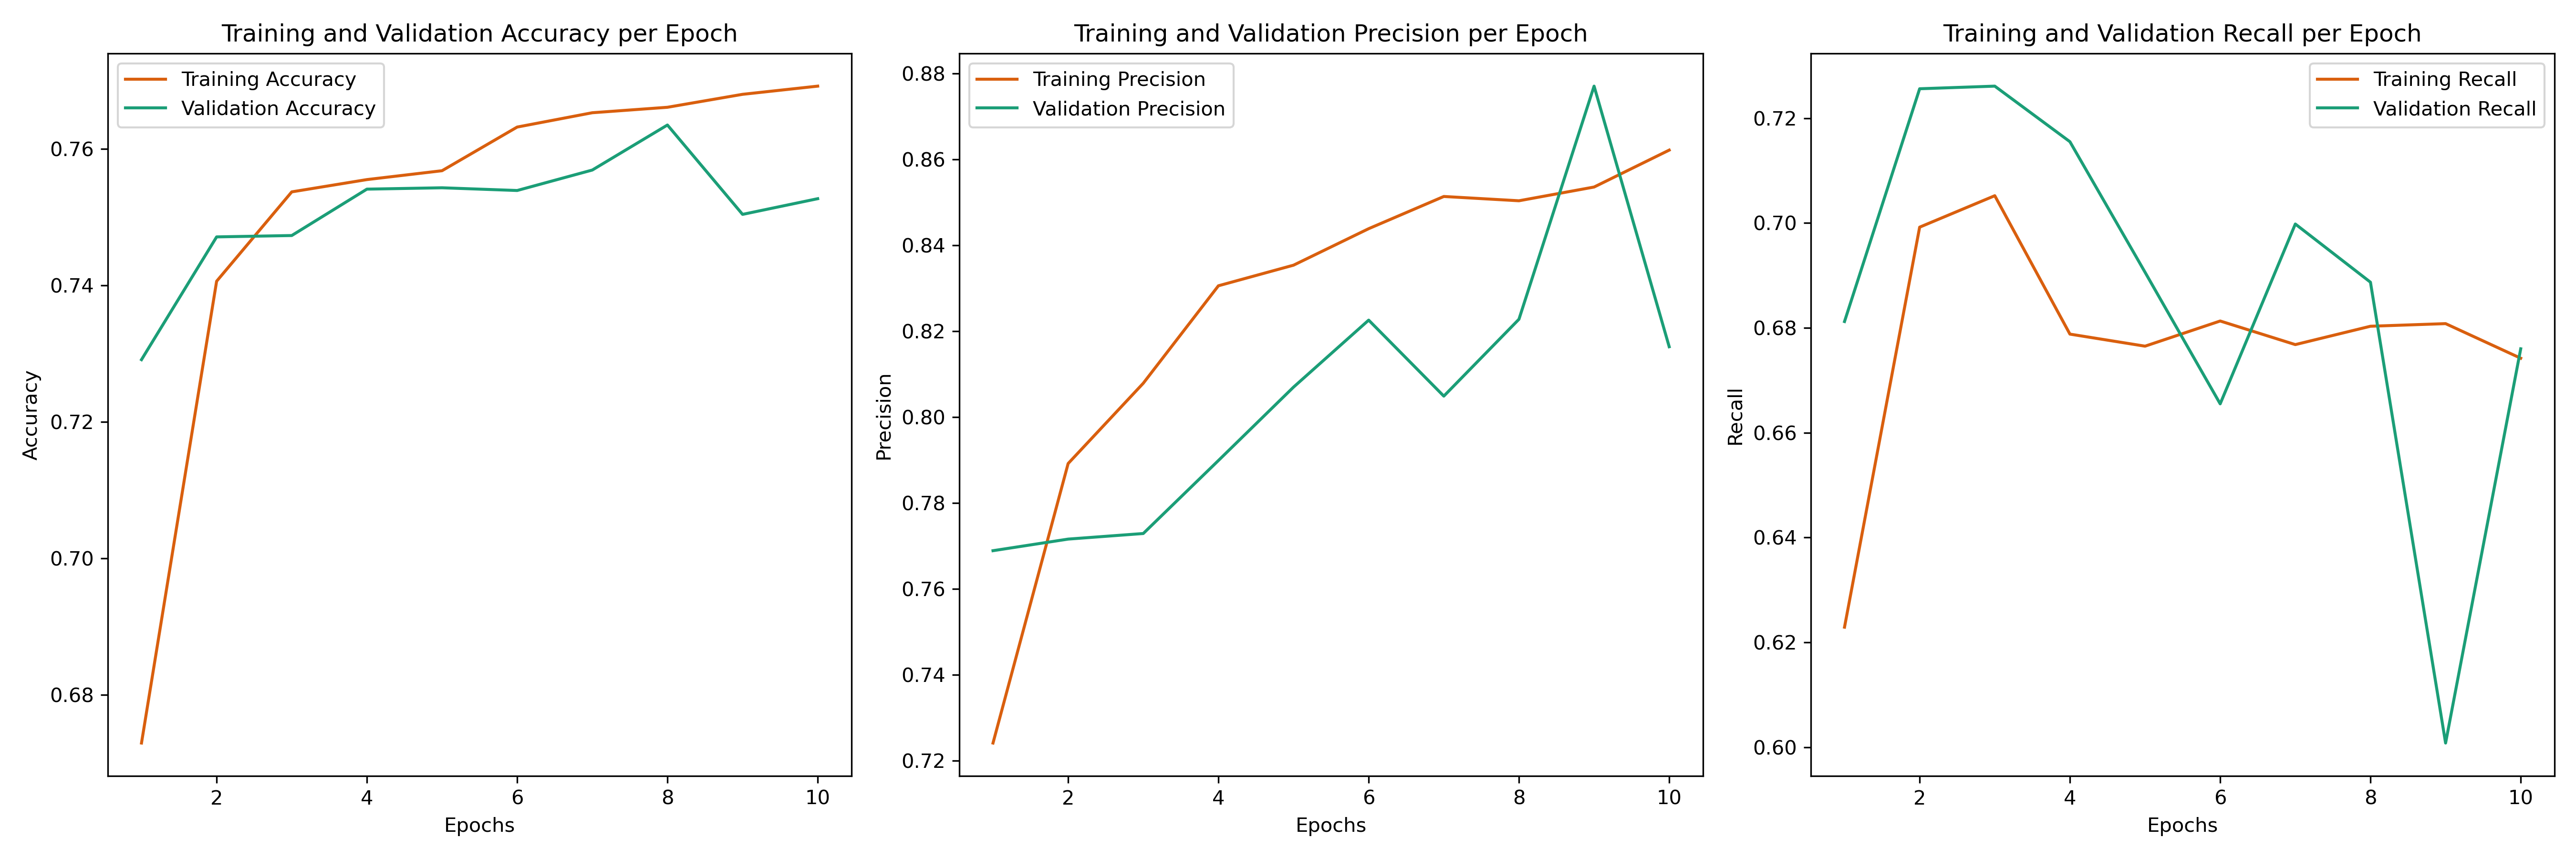
\includegraphics[width=0.9\textwidth]{wildfire_metrics.png}
    \caption{Graphic Representation of the Performance Metrics for the Training and Validation Sets Using VGG16 Across 10 Epochs.} \label{figvgg}
\end{figure}
On the validation set, the performance metrics also exhibited positive trends. The validation accuracy began at 0.7291 and varied across the epochs, reaching 0.7527 by the final epoch. Validation precision improved from 0.7689 in the first epoch to 0.8164 in the tenth epoch, while validation recall started at 0.6812 and ended at 0.6760.
\subsection{EfficientNet Implementation}
\begin{figure}[H]
    \centering
    \includegraphics[width=0.9\textwidth]{6channel.png}
    \caption{Representation of a 6 Channel RGB GeoTIFF Input. A: Representation of a 3-channel RGB GeoTIFF forested area \textit{before} a wildfire B: Visual example of a 3-channel RGB GeoTIFF forested area \textit{after} a wildfire.}. \label{fig1}
\end{figure}
EfficientNet \citep{tan2019} is a CNN architecture that uniformly scales network width, depth, and resolution with a fixed set of scaling coefficients. EfficientNet’s architecture begins with a base model, EfficientNet-B0, designed to find the optimal baseline network configuration. The following versions of the network are further scaled versions of B0, offering multiple models for different computational budgets. 

For this project, Efficient-B0 is adapted, trained, and tested using pre- and post-wildfire RGB GeoTIFF imagery pairs from the CWGID. To do this, an approach commonly known as Early Fusion (EF) is employed, where six-channel GeoTIFF files that combine the image pairs into a single input are built (see Figure \ref{fig1}). To use this, a custom function that allows the use of 6-channel GeoTIFF data with Efficient-B0 is built with the rasterio library and Keras' Sequence function (see Code \ref{lst:six_channel_generator}). 
\begin{lstlisting}[language=Python, caption={Custom Function to Feed Multi-Channel GeoTIFF Files to the EfficientB0 Model}, label= lst:six_channel_generator]
from keras.utils import Sequence
# Custom Data Generator for Six-Channel Images


class SixChannelGenerator(Sequence):
    # Change this depending on your own data
    # Initialize the generator
    def __init__(
        self,
        file_paths, # List of file paths to the six-channel GeoTIFF images
        labels, # Corresponding labels for the images
        batch_size=32, # Number of images to be returned in each batch
        dim=(256, 256), # Dimension of the images
        n_channels=6, # Number of channels in the images (6 in this case)
        shuffle=True, # Shuffle the data at the end of each epoch
    ):
        self.file_paths = file_paths
        self.labels = labels
        self.batch_size = batch_size
        self.dim = dim
        self.n_channels = n_channels
        self.shuffle = shuffle
        self.on_epoch_end()
    # Define the number of batches 
    def __len__(self):
        return int(np.ceil(len(self.file_paths) / self.batch_size))
    # Generate batch of data
    def __getitem__(self, index):
        # Generate indices of the batch
        batch_paths = self.file_paths[
            index * self.batch_size: (index + 1) * self.batch_size
        ]
        batch_labels = self.labels[
            index * self.batch_size: (index + 1) * self.batch_size
        ]
        # Initialize the arrays for the batch data and labels
        batch_x = np.empty(
            (len(batch_paths), *self.dim,
             self.n_channels), dtype=np.float32
        )
        batch_y = np.array(batch_labels, dtype=np.float32)
        # Load and read the data for each file in the batch
        for i, path in enumerate(batch_paths):
            with rasterio.open(path) as src:
		# Read the image and select the first 'n_channels' channels
                img = src.read()[: self.n_channels,
                                 : self.dim[0],
                                 : self.dim[1]]
		# Convert from channels_first to channels_last format
                img = np.moveaxis(img, 0, -1)
                batch_x[i,] = img / 255.0  # Normalize images to [0, 1] range

        return batch_x, batch_y
    # Shuffle the data at the end of each epoch
    def on_epoch_end(self):
        if self.shuffle:
            temp = list(zip(self.file_paths, self.labels))
            np.random.shuffle(temp)
            self.file_paths, self.labels = zip(*temp)
\end{lstlisting}

Furthermore, the data labeling and its use are formulated using the same pipeline as VGG16, by specifying the base paths to the training and testing directories for both damaged and undamaged classes. As above, the labeling of this model is based on the presence or the absence of ’Damaged’ in the imagery file paths.
 The base EfficientNet-B0 model is then loaded without its top layers (classification layers) and without pre-trained weights, as the pre-trained weights are specific to 3-channel images. A Global Average Pooling layer is used to reduce the spatial dimensions of the feature maps. To reduce overfitting, a Dropout layer is added with a specified rate of 30%


The model is built with an input tensor defined to accept 256px by 256px images with six channels. Initially, a standard convolutional layer is applied to this input tensor to perform an initial convolution operation, reducing it to a three-channel format. The base EfficientNet-B0 model is loaded both without the top layers (classification layers) and the pre-trained weights, as these were trained using 3-channel images. A Global Average Pooling layer is used to reduce the spatial dimensions of the feature maps. To reduce overfitting, a Dropout layer is added with a specified rate of 30\%. Following this, a dense layer is also added with 1024 neurons and ReLU activation (see Code \ref{lst:efficientnet_training}). In the end, the network outputs a probability indicating the likelihood of the image showing ’damaged’ versus ’undamaged’ areas.

\begin{lstlisting}[language=Python, caption={Initializing and Training EfficientNetB0 for Six-Channel Image Input}, label= lst:efficientnet_training]
from keras.layers import Input, Conv2D, Dense, GlobalAveragePooling2D, Dropout
from keras.models import Model
from keras.applications import EfficientNetB0
from keras.callbacks import EarlyStopping, ModelCheckpoint, ReduceLROnPlateau

# Model Adaptation for Six-Channel Input


# Change this depending on your own data
def create_efficientnet_six_channel(input_shape=(256, 256, 6), dropout_rate=0.3):
    input_tensor = Input(shape=input_shape)
    x = Conv2D(3, (3, 3), padding='same', activation='relu')(input_tensor)
    base_model = EfficientNetB0(
        include_top=False, input_tensor=x, weights=None)
    x = GlobalAveragePooling2D()(base_model.output)
    x = Dropout(dropout_rate)(x)
    x = Dense(1024, activation='relu')(x)
    output = Dense(1, activation='sigmoid')(x)
    model = Model(inputs=input_tensor, outputs=output)
    return model


# Initialize the model
model = create_efficientnet_six_channel()
# Model Training with Callbacks for Optimal Training Control
early_stopping = EarlyStopping(
    monitor='val_loss', patience=5, restore_best_weights=True)
model_checkpoint = ModelCheckpoint('yourmodel.keras', save_best_only=True)
reduce_lr = ReduceLROnPlateau(
    monitor='val_loss', factor=0.2, patience=2, min_lr=1e-6, verbose=1)

# Compile the model
model.compile(optimizer='adam',
              loss='binary_crossentropy',
              metrics=['accuracy', Precision(), Recall()])
\end{lstlisting}

Before training, class weights are calculated using the Scikit-learn library. Furthermore, Keras callbacks are set up for early stopping, model checkpointing, and reducing the learning rate when the validation loss plateaus, which helps optimize the training process. As VGG16, the model is compiled with the Adam optimizer and binary cross-entropy loss, with accuracy, precision, and recall as performance metrics.

For testing purposes, this EF architecture is trained on 23833 pre- and post-wildfire image pairs (divided as follows: 90\% for training and 10\% for validation) and is tested on 2716 pre- and post-wildfire image pairs. Training took around 930 minutes for 13 epochs. The detailed training and validation performance metrics for each epoch are provided in Table \ref{tab:1}. Furthermore, the graphs depicting the changes of the training and validation metrics over the 13 epochs can be seen in Figure \ref{figebo}.

\begin{table}[H]
    \centering
    \caption{Performance Metrics for Training and Validation Sets Using EfficientNetB0 Across Epochs. \label{tab:1}}
    \begin{tabular}{ccccccc}
    \toprule
\textbf{Epoch} & \textbf{Training Accuracy} & \textbf{Training Precision} & \textbf{ Training Recall} & \textbf{Validation Accuracy} & \textbf{Validation Precision} & \textbf{Validation Recall} \\
    \midrule
    1/13 & 0.7971 & 0.7204 & 0.4053 & 0.7843 & 0.7688 & 0.4973 \\
    2/13 & 0.8803 & 0.8299 & 0.6995 & 0.8703 & 0.7499 & 0.5754 \\
    3/13 & 0.8979 & 0.8599 & 0.7424 & 0.8152 & 0.8034 & 0.5404 \\
    4/13 & 0.9022 & 0.8668 & 0.7531 & 0.8179 & 0.7222 & 0.6024 \\
    5/13 & 0.9187 & 0.9016 & 0.7842 & 0.9125 & 0.7597 & 0.5647 \\
    6/13 & 0.9265 & 0.9156 & 0.8015 & 0.9310 & 0.7014 & 0.5948 \\
    7/13 & 0.9298 & 0.9181 & 0.8121 & 0.9363 & 0.7289 & 0.5726 \\
    8/13 & 0.9346 & 0.9260 & 0.8235 & 0.9359 & 0.7104 & 0.5946 \\
    9/13 & 0.9370 & 0.9274 & 0.8315 & 0.9057 & 0.7580 & 0.5464 \\
    10/13 & 0.9424 & 0.9387 & 0.8416 & 0.9291 & 0.7522 & 0.5835 \\
    11/13 & 0.9537 & 0.9590 & 0.8655 & 0.9333 & 0.9386 & 0.7959 \\
    12/13 & 0.9573 & 0.9644 & 0.8739 & 0.9363 & 0.9516 & 0.7959 \\
    13/13 & 0.9588 & 0.9665 & 0.8776 & 0.9333 & 0.9606 & 0.7757 \\
    \bottomrule
    \end{tabular}
\end{table}

During the training process, the model's performance on the training set showed a consistent increase in accuracy, precision, and recall. Specifically, the training accuracy improved from 0.7971 to 0.9588, precision increased from 0.7204 to 0.9665, and recall increased from 0.4053 to 0.8776 over the same period.

\begin{figure}[H]
    \centering
    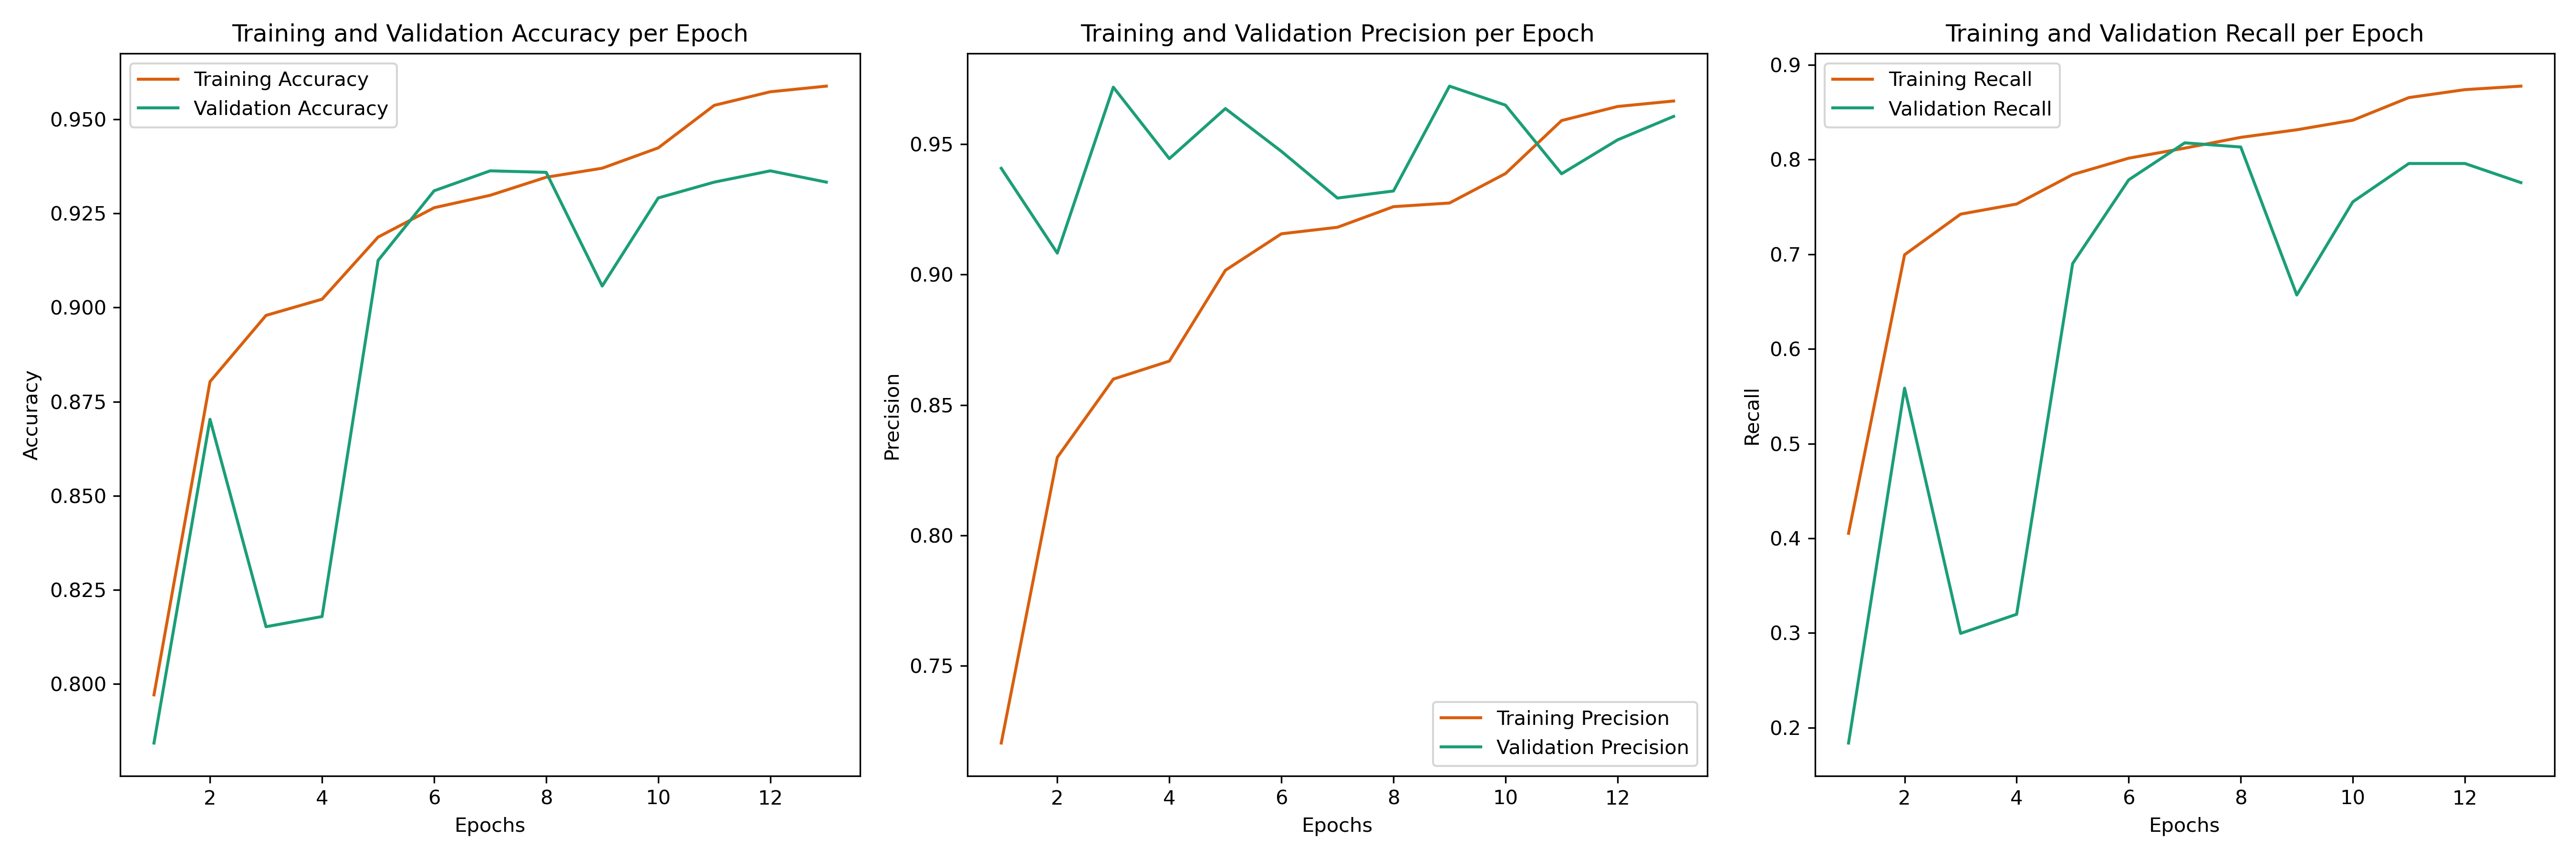
\includegraphics[width=0.9\textwidth]{wildfire_metrics_epoch_20.png}
    \caption{Graphic Representation of the Fluctuation of the Performance Metrics for the Training and Validation Sets Using EfficientNetb0 Across 13 Epochs.} \label{figebo}
\end{figure}

On the validation set, the performance metrics exhibited positive trends as well. The validation accuracy began at 0.7843, peaked at 0.9359 around the eighth epoch, and remained high at 0.9333 by the final epoch. Validation, precision, and recall also showed improvements, with precision starting at 0.7688 and reaching up to 0.9606, while recall improved from 0.497 to 0.7757.


\subsection{DL Results}
The results in Table \ref{tab:2} compare the performance of the two neural network architectures used on the CWGID. Each architecture's performance metrics are assessed, including loss, accuracy, precision, recall, and training time. Also, the percentage of the CWGID used to train each architecture is specified. 

Both models are trained with subsets of the CWGID dataset, with the 6-channel input EF EfficientNet model and the VGG16 model using around 25\% of the data. 

The 6-channel input EfficientNet achieved the lowest loss (0.178) and highest accuracy (92.6\%), making it the most effective model in terms of overall performance. Its precision was at 92.5\% and its recall was 81.9\%, indicating a strong ability to identify damaged areas correctly with some missed detections. 

VGG16, had a higher loss (0.718) with an accuracy of 76.4\%. Its precision was 83.7\% and its recall was 68.9\%. This architecture took a longer training time of 1010 minutes compared to 930 minutes for the EfficientNet model. The EfficientNet model shows a slight faster training time when considering the amount of training epochs.

The 6-channel input EfficientNet demonstrated superior performance in accurately classifying areas affected by wildfires with high precision and accuracy, making it an efficient choice for applications where accurate assessments are critical. Moreover, it is important to mention that VGG16 was tested with 6-channel inputs but proved computationally intensive.
 

 \begin{table}[H]
    \centering
    \caption{Performance Metrics of the Models. \label{tab:2}}
    \begin{tabular}{ccc}
    \toprule
    \textbf{Model} & \textbf{6-channel input EfficientNet} & \textbf{VGG16} \\
    \midrule
    Data from the CWGID (\%) & 25 & 25 \\
    Loss & 0.178 & 0.718 \\
    Accuracy & 0.926 & 0.764 \\
    Precision & 0.925 & 0.837 \\
    Recall & 0.819 & .689 \\
    Time (minutes) & 933 & 1010 \\
    \bottomrule
    \end{tabular}
\end{table}
\section{Discussion}

The methodology developed in this study facilitates the creation of large, reliable, and cloud-free bi-temporal satellite imagery datasets, which are essential for accurate environmental monitoring. Also, by leveraging historical and curated datasets for the labeling, our approach maximizes the value of existing data, accurately labels the imagery, and minimizes the need for manual labeling.

Furthermore, the methodology was successfully evaluated, as the CWGID enabled the adapted CNN models to learn and identify the signs of wildfire damage with high accuracy, specifically with the EF EfficientNet-B0 model. Additionally, the proposed methodology produced a greater number of examples compared to other similar datasets in the field \citep{al-dabbagh2023uni,SEYDI2022108999,Hunan}, which can boost the performance of deep learning models, making them more effective at detecting and analyzing environmental changes. Moreover, the high precision and recall metrics for EfficientNet, particularly the recall of 81.9\%, display the model’s capacity to correctly identify wildfire-affected areas with fewer false negatives, which remains critical for rapid and effective wildfire monitoring.

On top of that, the dataset's bi-temporal collection of pre- and post-wildfire satellite imagery also offers the possibility to use different and accurate approaches for detecting forest wildfires with satellite imagery. The comparative analysis of VGG16 and EfficientNet shows the advantage of employing a bitemporal approach to satellite imagery analysis under a single input. By evaluating \textit{before} and \textit{after} images as coupled inputs, the model identifies changes that a single post-event imagery might not reveal, as shown by VGG16. 


\section{Conclusion}

This paper illustrates a Python methodology that integrates DL with satellite imagery to enhance environmental monitoring. Specifically, the development of the California Wildfire GeoImaging Dataset (CWGID) and its evaluation using DL architectures are outlined. The approach explained throughout this work allows for accurate detection of forest wildfires, as demonstrated using DL architectures, and can be applied to a broad range of environmental issues beyond just wildfire detection.
Firstly, historical data, Python-based tools, and Google Earth Engine are leveraged to build and label a large, cloud-free Sentinel-2 satellite imagery dataset depicting forest wildfire examples. Then, this dataset is used to train well-known CNN architectures, enabling the effective detection of forest wildfires within the satellite imagery. An accuracy of 92.6 \% with the EfficientNetB0 model was obtained, indicating the potential effectiveness of the methodology.
Future studies will include using Fully Convolutional Networks (FCNs), like U-Nets \citep{DBLP:RonnebergerFB15}, because they allow pixel-wise classification. It is anticipated that these networks will enhance the accuracy of detecting and mapping wildfire-affected areas, leveraging the detailed ground truth masks included within the CWGID.


\bibliography{mybib}
\bibliographystyle{unsrtnat}



